\section{System Architecture}

The system implements a modern, decoupled client-server architecture designed for scalability and maintainability. It is composed of three primary layers: the Frontend Client, the Backend API Server, and a specialized Worker Service for heavy asynchronous processing.

\begin{figure}[H]
    \centering
    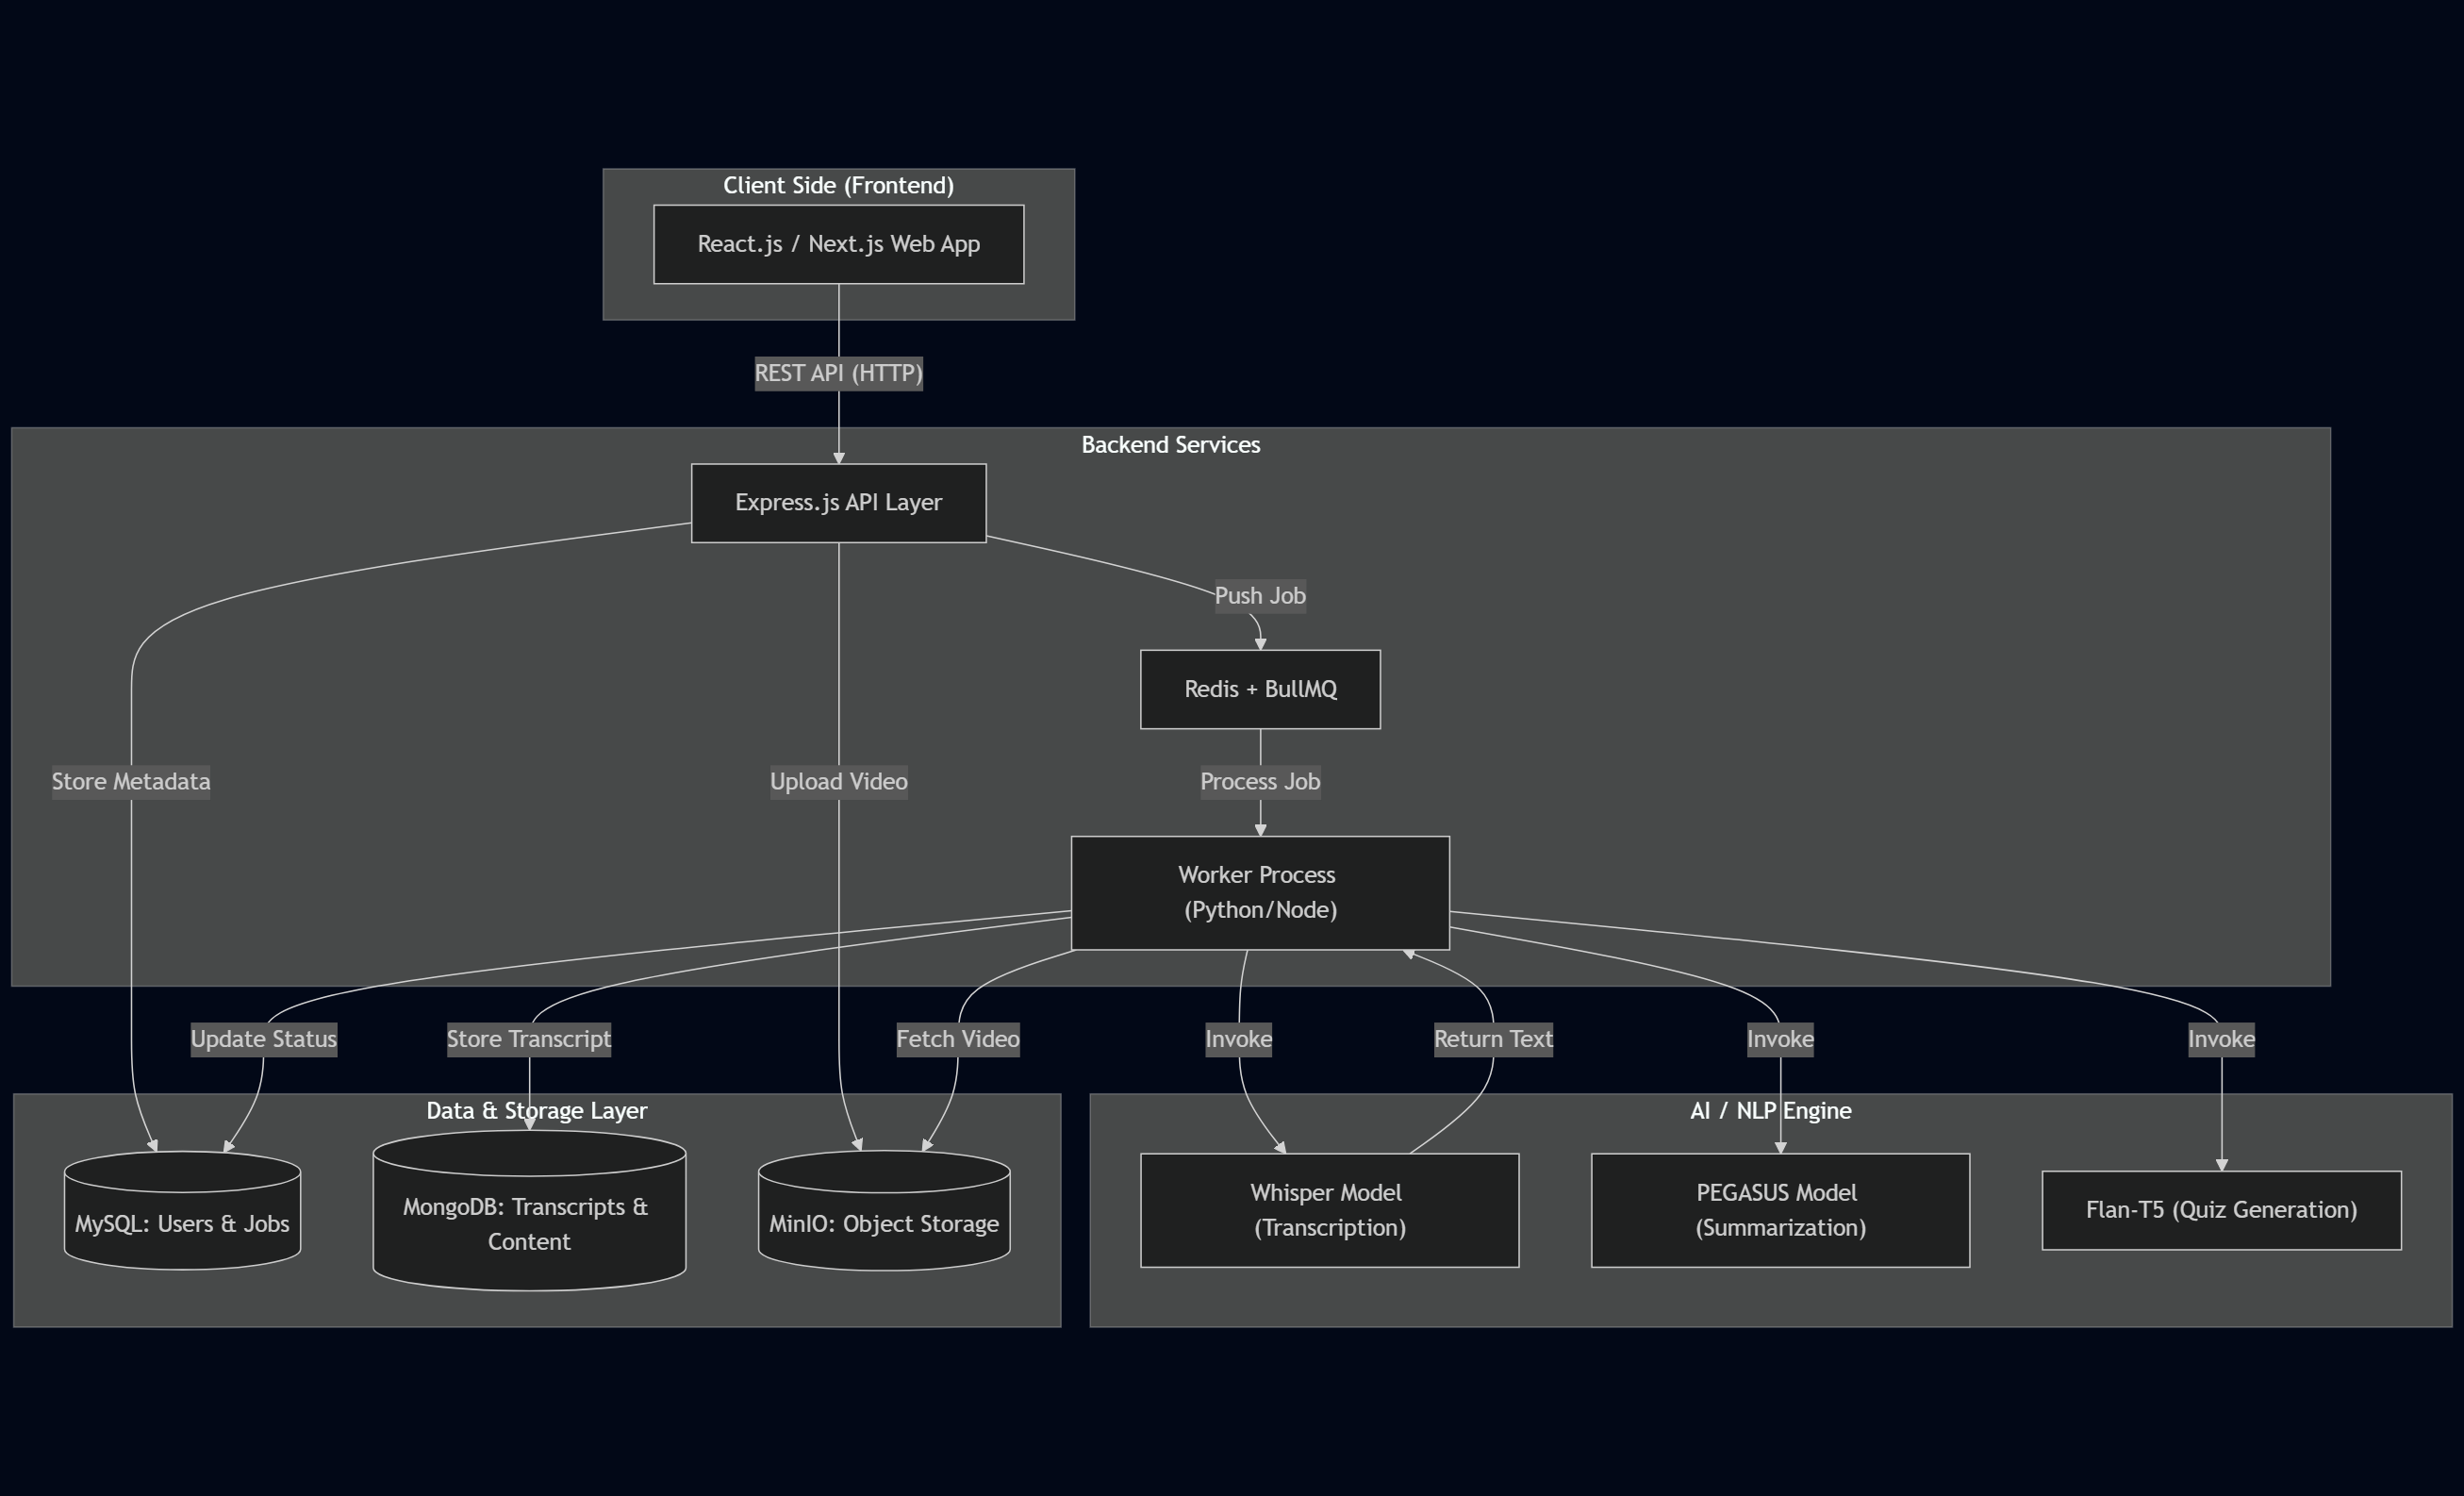
\includegraphics[width=1.0\linewidth]{system/images/1. System_Architecture_Diagram.png}
    \caption{System Architecture Diagram}
    \label{fig:system_architecture}
\end{figure}

\subsection{Frontend Layer}
The user interface is built using Next.js, a React-based framework that enables server-side rendering (SSR) and static site generation (SSG). This choice ensures high performance, SEO optimization, and a seamless user experience. Key responsibilities of the frontend include:
\begin{itemize}
    \item Efficient page rendering and asset management.
    \item File upload management with progress tracking.
    \item Real-time video playback with synchronized captions.
    \item Interactive transcript viewing and summary display.
\end{itemize}

\subsection{Backend Layer}
The core application logic is hosted on a Node.js server running Express. This layer exposes a RESTful API that handles:
\begin{itemize}
    \item Request validation and routing.
    \item Coordination between storage services and the processing queue.
    \item Secure generation of presigned URLs for media access.
\end{itemize}

\subsection{Asynchronous Processing Layer}
To ensure the application remains responsive during computationally expensive tasks, the system utilizes an asynchronous worker pattern.
\begin{itemize}
    \item BullMQ \& Redis: Manages a reliable job queue ("transcribe"). Jobs are enqueued by the API and consumed by independent workers.
    \item Worker Service: A dedicated Node.js process that orchestrates the execution of AI models.
    \item AI Subsystems:
        \begin{itemize}
            \item Whisper: Performs robust speech-to-text transcription.
            \item LED (Longformer Encoder-Decoder): Generates abstractive summaries from the transcripts.
            \item Two-stage MCQ pipeline: A question generation model paired with a distractor generation model produces complete multiple-choice questions from the transcript.
        \end{itemize}
\end{itemize}

\subsection{Data Storage Layer}
The system leverages a polyglot persistence strategy to efficiently handle different data types:
\begin{itemize}
    \item MySQL: Stores structured relational data such as job status, user accounts, and quiz metadata.
    \item MongoDB: Stores semi-structured and unstructured data, including full transcripts and generated summaries.
    \item MinIO: An S3-compatible object storage service used for hosting large video and audio assets (serving as a staging solution for future AWS S3 migration).
\end{itemize}
